%% NB: conversation with Helen Hanlon - suggested that 10 years overlap period is not really enough o be capture sufficient natural variability (problem not to do with sample size - so including more grid cells doesnt really help with this).
% One idea would be to do an additional comparison over a longer period between aggregated daily values form 2.2km model and CEH-GEAR Daily.

% \documentclass[APA,STIX2COL]{WileyNJDv5}
\documentclass[APA,Times2COL]{WileyNJDv5}
\usepackage{geometry}
\usepackage[parfill]{parskip}
\usepackage{tabularx}
\usepackage{booktabs}
\usepackage{lscape}
\usepackage{enumitem}
\usepackage{subcaption}
\usepackage[demo]{graphicx}
% \usepackage[table,xcdraw]{xcolor}
% \usepackage{amsmath}
% Include numbering for {paragraph|}
% \setcounter{secnumdepth}{4}
\usepackage{fontspec}
\usepackage{todonotes}
\usepackage{afterpage}

\usepackage[utf8]{inputenc}
 
\usepackage[round]{natbib} % "round" will make the brackets like this: ()
\bibliographystyle{wileyNJD-APA.bst}
% \bibliographystyle{ajs.bst}

% \newcolumntype{C}[1]{>{\centering\arraybackslash}p{#1}}
\newcolumntype{L}[1]{>{\raggedright\let\newline\\\arraybackslash\hspace{0pt}}m{#1}}
\newcolumntype{C}[1]{>{\centering\let\newline\\\arraybackslash\hspace{0pt}}m{#1}}
\newcolumntype{R}[1]{>{\raggedleft\let\newline\\\arraybackslash\hspace{0pt}}m{#1}}

% \setlength{\belowcaptionskip}{-10pt}
\graphicspath{{Figures/}} % Location of the graphics files

\title{\textbf{The sensitivity of urban surface water flood modelling to the temporal distribution of rainfall}}
\date{}
% \author{Molly Asher}

\geometry{verbose,tmargin=1cm,bmargin=3cm,lmargin=2cm,rmargin=2cm}

\begin{document}
\maketitle
\vspace{-1.5cm}
% \pagestyle{empty}
\pagenumbering{arabic}

\section{Abstract}

The risk posed globally by surface water flooding to people and properties is growing due to rapid urbanisation, infrastructure development and intensification of rainfall. Whilst tools to model urban flood risk have also been rapidly developing, there remains a knowledge gap around the sensitivity of urban hydraulic modelling methods to the temporal structure of rainfall. In the UK, the industry standard process considers rainfall events to always be symmetrical, and with a singular peak in intensity. Extensive study of UK extreme rainfall events suggests that loading of rainfall towards the start or end of events is in fact more common. In the present study, the sensitivity of two urban catchments in the north of England are tested using fifteen realistic profiles derived from these observed extremes. Additionally, systematic variations are made to the industry standard profile to shift the single peak towards the start or end of the event. We demonstrate that the positioning of the peak, as well as its magnitude, influences the severity, timing and nature of the associated flooding. The profile with the latest peak results in an 18\% larger flooded area than the early peaking profile causing the smallest flooded area.

\todo[inline]{Update the stats at the end and add additional key stats.}

\section{Introduction}\label{sec:introduction}

Flooding is now the most frequently occurring and harmful natural hazard globally \citep{jenkins2018probabilistic, razavi2020anthropocene}. In the UK, the largest share of this overall flood risk comes from surface water flooding \citep{houston2011pluvial}. Surface water flooding occurs when the volume of rainfall exceeds the absorption capacity of the ground and the storm water drainage capacity \citep{archer_characterising_2015}. It generally occurs in urban settings which tend to have a higher proportion of impermeable surfaces which preclude the natural processes that moderate floods in rural environments. Surface water flooding is thus more directly dependent than other flood sources on the characteristics of rainfall \citep{ochoa2015impact}. Understanding and accurately representing these dynamics is of paramount importance for accurate surface water flood risk modelling.

Flood modelling, like all forms of modelling, necessitates the use of simplifications to make complex natural phenomena manageable and comprehensible within computational frameworks. This simplification process involves making certain assumptions and approximations to represent the real-world processes that govern flooding. One notable simplification concerns the representation of rainfall \citep{bardossy2022precipitation}. Rainfall in models is commonly represented using design storms which are idealised rainfall events with simplified characteristics \citep{butler_urban_2004}. Design storms are advantageous as they avoid the need to model multiple individual historical rainfall events in a particular catchment and allow a standardised approach to assessing the impact of extreme rainfall \citep{balbastre2019comparison, marsalek1984design}. The total event rainfall depth is calculated through statistical analyses of historical rainfall data, and this rainfall depth can be tailored to different durations and return periods. This depth is then distributed over time using a hyetograph which represents the time varying distribution of rainfall during a storm. The way in which the hyetograph is specified, and the impact of this on the resulting flood risk, is the focus of this work.

In the UK, the Flood Studies Report (FSR) and its successor, the Flood Estimation Handbook (FEH), have established a robust and widely accepted approach to flood modelling since the FSR was first published in 1975. Following this, the industry standard approach to flood risk modelling advises use of one of two design hyetographs specified in the FSR. These profiles are both symmetrical with a central peak in intensity. They are to be applied irregardless of the event duration or return period, with a summer profile, which is more sharply peaked, advised for use in urban areas, and a winter profile, which has a more shallow peak, recommended for rural catchments \citep{faulkner1999}. 

There are a number of different approaches to specifying hyetographs. These are outlined in detail by \citet{chow1988applied}, \citet{veneziano1999best}, and \citet{balbastre2019comparison}, amongst others. The approaches can be loosely categorised as: observed (directly using temporal distributions from observed events); summary (generalising temporal distributions from observed events); stochastic (utilising stochastic rainfall models); or IDF curve-based methods (using rainfall characteristics from IDF (intensity duration frequency) curves alongside simple distribution shapes). The FSR profiles are best described as summary hyetographs, and were derived by study and generalisation of just 80 summer (May to October) and 32 winter (November to April) storms of 24-hour duration occurring between 1961 and 1970. The generalisation process is described in detail by Villalobos-Herrera (in press?). Importantly, in addition to the stages typical of generating summary hyetographs, an extra procedure is carried out which involves shifting each observed event's peak intensity to the centre. This ensures that when summary profiles are derived from averaging across multiple observed rainstorms, there is always a temporally central peak in intensity. Whilst much of the flood estimation methods associated with the FEH have been updated since the FSR's original release, the hyetographs have not been revised in the last fifty years. 

% Old evidence, and process that obfuscates temporal variability

Recent research indicates that the FSR hyetographs are not representative of the true variety in the timing of peak intensity in observed storms. A set of $\sim$70,000 UK independent rainstorms ranging from sub-hourly to daily durations were identified by \citet{herrera2023creation} using a new storm identification algorithm. These storms were used to trial an alternative approach to deriving summary hyetographs which removes the centring step applied in the FSR methodology. Rather, the positioning of the peak is made integral to the hyetograph classification, with profiles classed as front loaded, centred or back loaded. Importantly, Villalobos-Herrera et al. (?) identify using this method that just 23\% of the observed storms have a central peak in intensity. This provides evidence that the majority of UK extreme storms are fundamentally different to design storms produced with the FSR hyetographs, and calls into question the validity of their continued application in UK flood modelling approaches. 

% This provides evidence that the majority of UK extreme storms are fundamentally different to design storms produced with the FSR hyetographs. This paper aims to build on this finding and to provide evidence on the extent to which this misrepresentation translates into significant differences in the flooding outcomes 

% this fundamental misrepresentation of storm temporal profiles translates into a significant difference in flooding outcome. 

This paper aims to build on this finding and to provide evidence on the extent to which hydrological response in a UK catchment shows sensitivity to this misrepresentation of storm temporal profile. The sensitivity of hydrological response to the temporal structure of rainfall is already evidenced in multiple studies. The majority of these studies focus on the impact of temporal profiles on flood peak discharge (\citet{fatone2021advanced}, \citet{dullo2017evaluation}, \citet{maca2009influence}, \citet{fadhel2018sensitivity}, \citet{wasko2015steeper}), in some cases with concurrent analysis of changes to the flood volume (\citet{lambourne1987model}, \citet{nguyen2010optimal}, \citet{peyron2002optimal}) or the time to peak (\citet{balbastre2019comparison}, \citet{ball1992influence}). Other studies have focused on flood depth alone \citep{hettiarachchi2018increase}, or more specific indicators, including the manhole overflow inundation area \citep{li2021case}, drainage system performance factors \citep{ng2020design}, and the capacity required in a storm water reservoir  \citep{pochwat2017temporal}. 

This existing research on storm temporal profiles and their impact on flooding outcomes leaves two notable gaps. First, while studies applying idealised profiles have tested a variety of simple, summary temporal patterns, they have often failed to conduct systematic adjustments to these profiles to assess the consequences of shifting the timing of the peak intensity. Second, there is an absence of research examining realistic observed rainfall profiles within the context of the UK. These two gaps underscore the need for further investigations to comprehensively analyse how variations in peak timing, both in idealised and real-world scenarios, influence flood risk assessments in urban catchments. The recent evidence produced by Villallobos-Herrera et al (in press) on the range of observed profiles present in UK extremes, presents an opportune moment to address these gaps. 

Specifically, the aims of this paper are to use rain-on-grid flood modelling to test the sensitivity of flooding in an urban catchment to:

\begin{enumerate}
  \item The timing of the peak intensity in an idealised, single-peaked design storm (based on the FSR summer profile)
  \item The range of temporal distributions in physically realistic hyetographs, and to quantify how these outcomes differ from using a single-peaked design storm (based on the FSR summer profile)
\end{enumerate}


\section{Methods}\label{sec:methods}
\subsection{The flood inundation model}\label{subsec:model:catchments}

A 2D hydraulic rain-on-grid model is run in Hec-Ras 6.4.1 using the 2D unsteady diffusion wave equation set. The model takes a rainfall input and simulates the movement of this water overland, according to the topography, defined with a Digital Elevation Model (DEM). In this work, the DEM is based on 1m 2019 composite LIDAR data (Environment Agency, 2020), with the `bare earth' terrain data modified to include hydraulic structures and buildings (Houston et al, 2011). 

\todo[inline]{This is for Lin Dyke - need to find out about DTM for Wyke Beck. Also difference in resolution - 1m2 vs 2m2}

The model is supplied with a six hour duration rainfall input. and then is run for a total of 70 hours to ensure that the hydrology processes happening in the catchment after the storm are adequately captured. The computation time step is variable and automatically adjusted to ensure the Courant value remains between 0.75 and 2 (as reliable results are associated with a Courant value as close to 1 as possible).

% Limitations include the assumptions made in the data such as, no losses due to urban drainage, the variation in hydraulic roughness, and the resolution of the DTM.

\subsection{The study catchments}\label{subsec:model:catchments}

Wyke Beck and Lin Dyke are two suburban catchments on the eastern edge of Leeds, in the north of England (Figure \ref{fig:catchment_locations}). Lin Dyke has an area of 22.9km \textsuperscript{2}: this includes urban and suburban land uses around the settlements of Kippax and Garforth (27\% of total catchment area); rural land uses including a large amount of arable land, and some woodland and grassland (69\% of total catchment area); and water, including an area of wetlands in the southern reaches, and some small streams draining into the river Aire at the catchment's southern end (4\% of total catchment area). 
Wyke Beck is slightly bigger at 33.6km \textsuperscript{2}, and includes: a large urban proportion containing numerous populous Leeds suburbs (63\% of total catchment area); rural land uses, including grassland and woodland (36\% of total catchment area); and water, including Waterloo Lake to the north of the catchment and Wyke Beck, a tributary of the river Aire (1\% of total catchment area) (Figure \ref{fig:catchment_landcover}). 

\todo[inline]{Add description of topography and climate in catchments? Double check land cover data, Wyke Beck in particular i think is dodgy. Should we mention that land cover classes for Lin Dyke don't seem to cover all of the areas of permanent water.}

% \begin{figure}[h!]
\begin{figure*}[!t] 
\centering
\begin{subfigure}[H]{0.45\linewidth}
   \centering
   \includegraphics[width=\linewidth]{Figs/Catchment/BothCatchmentsLocation.PNG}
   \caption{Location of catchments in the wider Leeds area }
   \label{fig:catchment_locations}
\end{subfigure}
\\[\baselineskip]
\begin{subfigure}{0.45\linewidth}
   \centering
   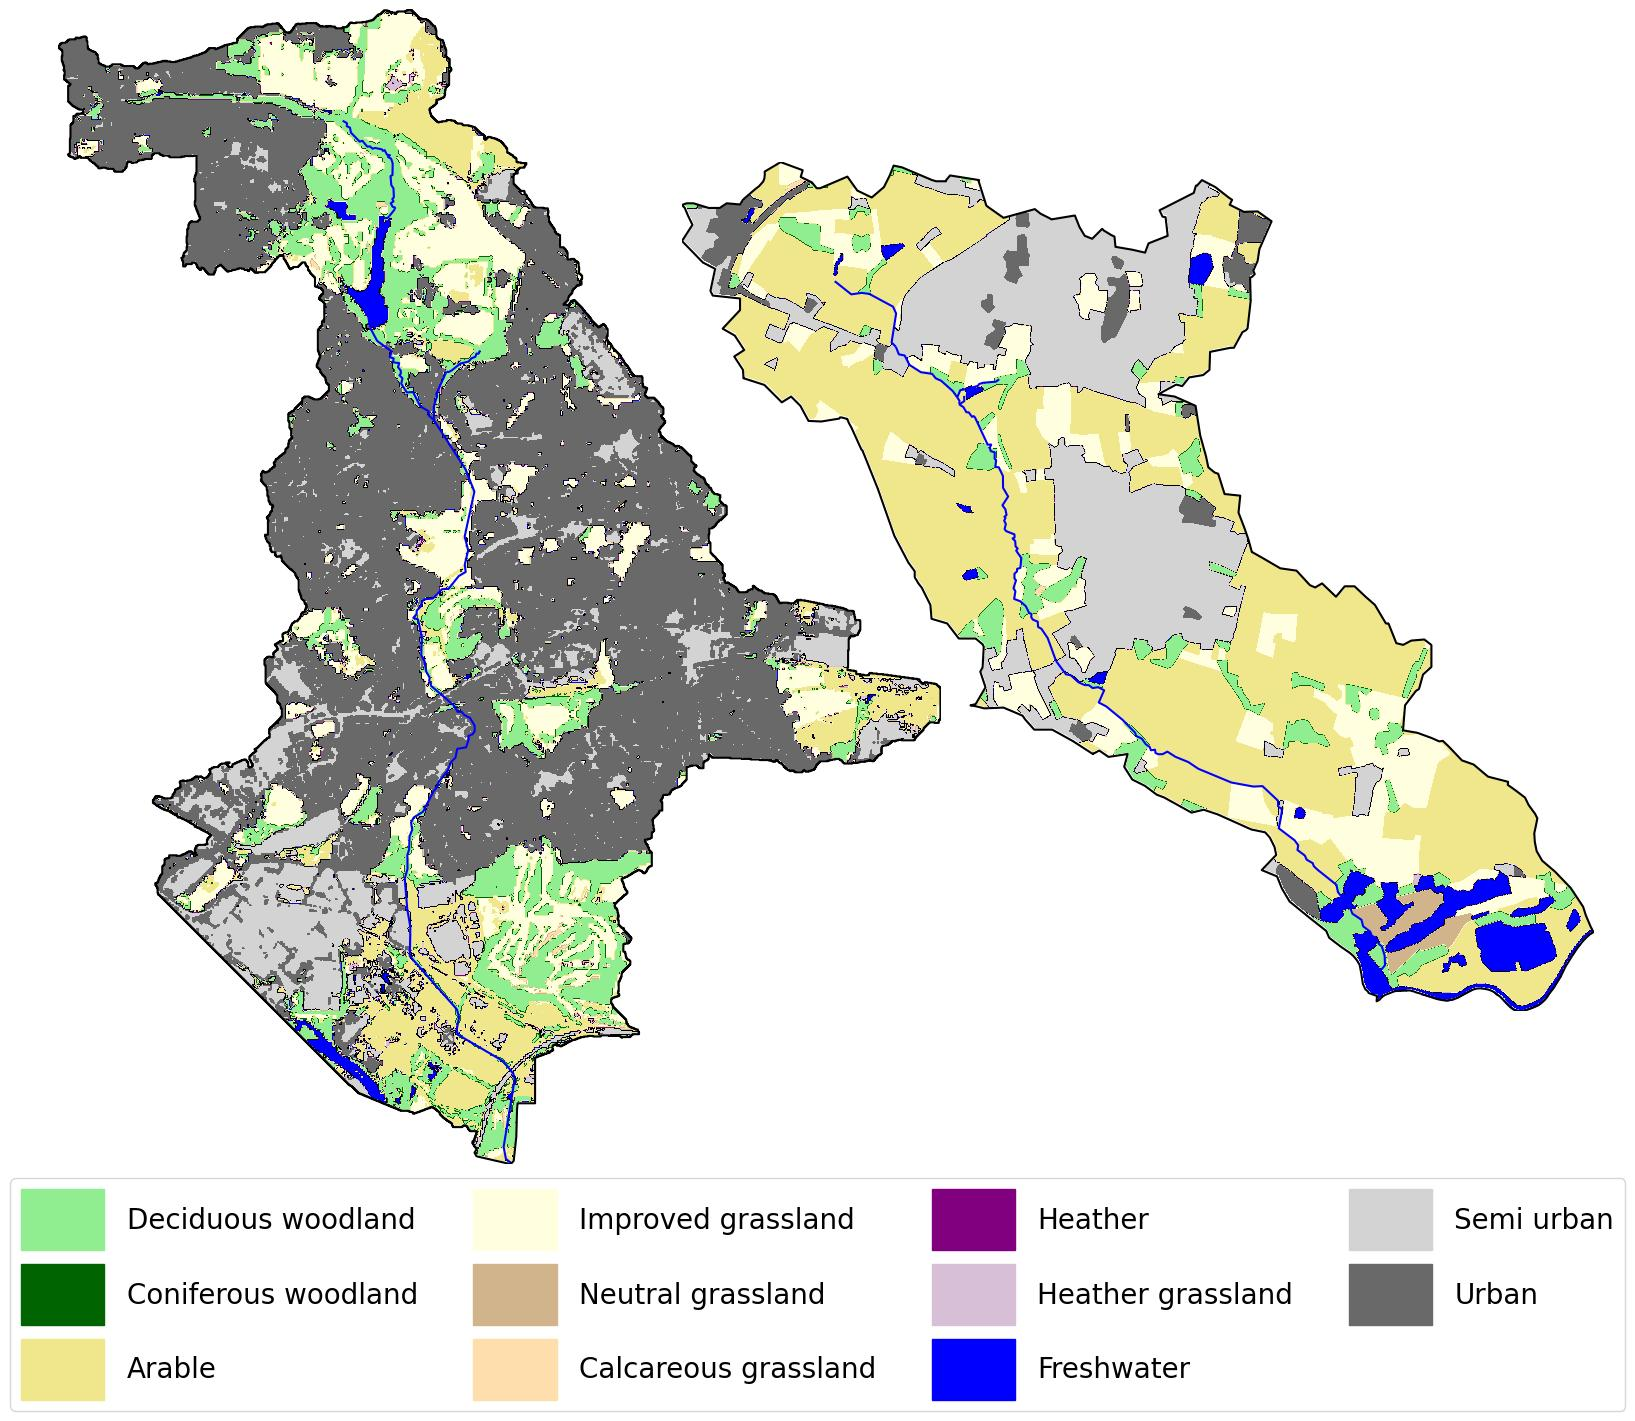
\includegraphics[width=\linewidth]{Figs/Catchment/LandCover_BothCatchments.jpg}
   \caption{Land use}
   \label{fig:catchment_landcover} 
\end{subfigure}
\hfill
\begin{subfigure}{0.45\linewidth}
   \centering
   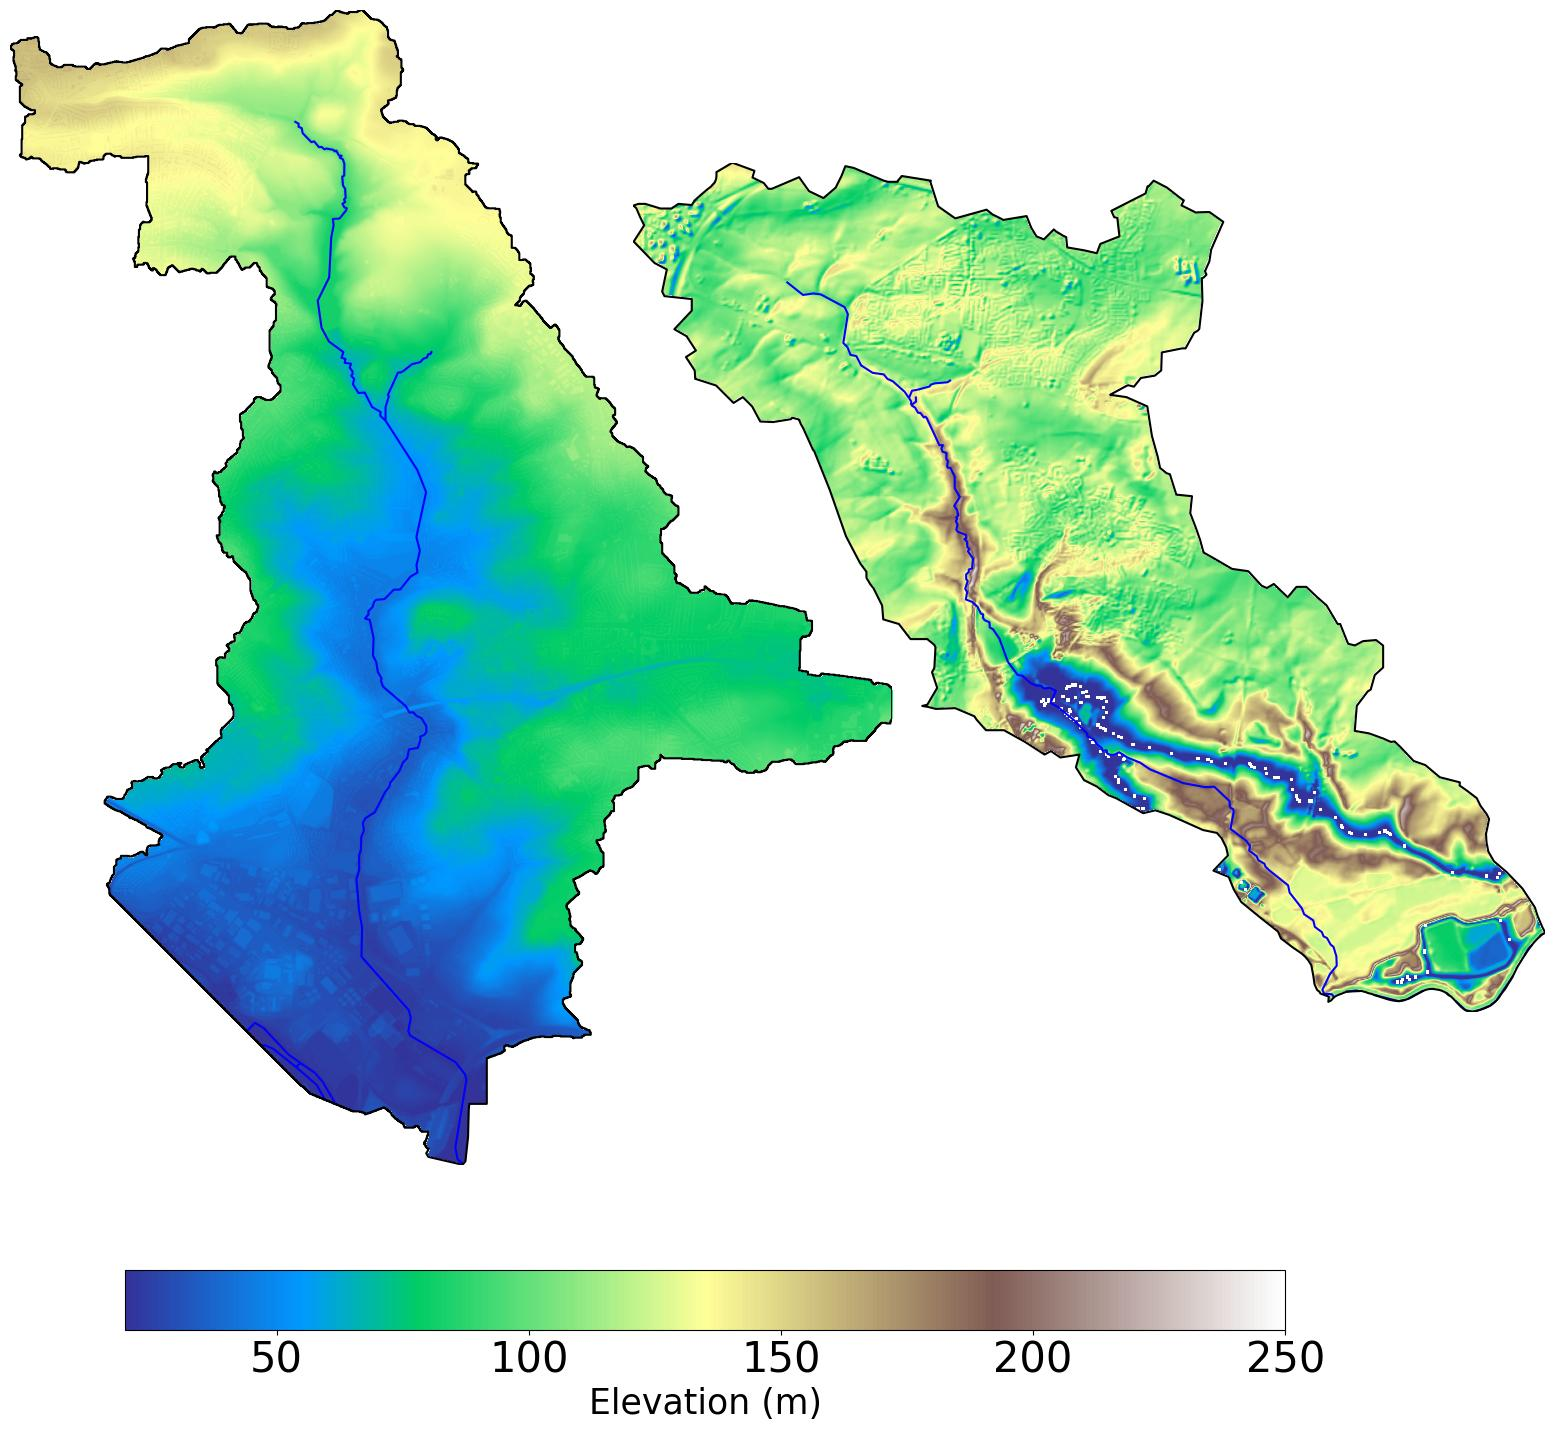
\includegraphics[width=\linewidth]{Figs/Catchment/Terrain_BothCatchments.jpg}
   \caption{Topography}
   \label{fig:catchment_terrain}
\end{subfigure}
\centering
\caption{Wyke Beck (left) and Lin Dyke (right)} \label{fig:catchments} 
\end{figure*}


\todo[inline]{Add to top plot showing location within England}

\subsection{The rainfall data}\label{sec:rainfalldata}
In the UK, the Flood Estimation Handbook (FEH) is the industry standard for assessing flood risk. The FEH web service provides rainfall depths associated with specific durations and return periods for UK catchments. These depths are estimated from historical rainfall data and a depth duration frequency (DDF) model. The rainfall depth associated with a 6 hour duration, 1-in-100 year return period event in each of the two catchments is used here. For Lin Dyke this is a depth of 59.29mm and for Wyke Beck it is 59.25mm. 

Design storm profiles are required to translate this rainfall depth into the hyetographs which form the rainfall input to the flood model. The focus of this work is on the impact of the shape of these design storm profiles. A hyetograph was produced for each catchment using the FSR summer design profile, following the industry standard approach, and then additionally two alternative sets of design storm profiles were developed and applied to the model, as described below.

\subsubsection{Idealised profiles}
A set of nine idealised profiles were derived through first approximating the method used to construct the FSR summer design storm profile, and then applying systematic variations to shift the peak in time (Figure \ref{fig:profiles}, top left and Table \ref{table:profile_names}).

The centred, symmetrical FSR profile is produced using Equation \ref{eqn:fsr}, where the proportional depth of rain, $y$, falling in the temporal proportion, $x$, of the total duration, centred on the peak is given as:

\begin{equation}
\text{y} = \frac{1-a^{z}}{1-a}
  \label{eqn:fsr}
\end{equation}

where \textit{z} = $x^b$, and $a$ = 0.100 and $b$ = 0.815 for the summer profile. 

It is a known limitation of this formula that it gives unrealistically large values for the 50\% summer profile when a large number of time steps are used. However, despite amendments being made to this formula since its initial publication, no supporting documentation of the implemented amendments are openly offered. Consequently, our approximation of the FSR rainfall curve has a slightly sharper and higher peak, and this presents a small limitation in our work. 

Eight further idealised profiles were then created by shifting the peak of this approximated FSR summer profile in time. Four versions are front loaded (with the peak in intensity occurring during the first half of the event) and four are back loaded (with the peak in intensity occurring during the second half of the event). This was done...  The magnitude of the peak is conserved across all profiles, allowing the influence of the timing of the peak to be investigated, decoupled from the influence of the magnitude of the peak. 

\todo[inline]{Add info above on how we shifted the peak in time}

\begingroup
\setlength{\tabcolsep}{10pt} % Default value: 6pt
\renewcommand{\arraystretch}{1.5} % Default value: 1
\begin{table*}[h!]
\centering
\caption{Abbreviations used for idealised and observed profiles}
\begin{tabular}{cccc} 
 \hline
 \textbf{Title} & \textbf{Description} & \textbf{Idealised Profiles} & \textbf{Observed Profiles} \\ [0.5ex] 
 \hline
 Very front loaded & Max intensity first 20\% & I1, I2 & O1, O8, O15\\
 Front loaded & Max intensity second 20\% & I3, I4 & O3, O11, O10 \\
 Centred & Max intensity middle 20\% & I5 & O6, O9, O13\\
 Back loaded & Max intensity second last 20\% & I6, I7 & O2, O12, O14\\
 Very back loaded & Max intensity last 20\% & I8, I9 & O4, O5, O7\\[1ex] 
 \hline
\end{tabular}
\label{table:profile_names}
\end{table*}
\endgroup


\subsubsection{Observed profiles}
A further fifteen summary profiles defined from analysis of observed extremes were tested (Figure \ref{fig:profiles}, top right, and Table \ref{table:profile_names}). The method for producing these summary profiles is described in detail by Villalobos-Herrera (202X). The profiles describe the proportion of the total rainfall depth which falls within each of twelve time steps for any event duration. The total rainfall depth falling in each time step is assumed to fall at a constant rate. Thus, a six hour duration event is comprised of twelve time steps of 30 minutes each, with each minute assigned a rainfall depth of 1/30th of the time step total. The time step total is calculated by multiplying the total event rainfall for a six hour event (as calculated in Section \ref{sec:rainfalldata}), by the proportion of rainfall assigned to that time step.  

The variation in the magnitude of the peak intensity between these profiles makes drawing conclusions about the impact of the timing of the peak harder. However, these profiles do allow quantification of the magnitude of the difference in flooding outcomes between profiles which are physically realistic. 


\begin{figure}[!t] 
\centering
\begin{subfigure}[H]{\linewidth}
   \centering
   \includegraphics[width=\linewidth]{Figs/Profiles/Idealised_Observed_Profiles_LinDyke_prelossremoval.png}
   \caption{Pre loss removal}
   \label{fig:prelossremovalprofiles}
\end{subfigure}
\\[\baselineskip]
\begin{subfigure}{\linewidth}
   \centering
   \includegraphics[width=\linewidth]{Figs/Profiles/Idealised_Observed_Profiles_LinDyke_postlossremoval.png}
   \caption{Post loss removal }
   \label{fig:postlossremovalprofiles} 
\end{subfigure}
\hfill
\centering
\caption{Hyetograph profiles used in model sensitivity testing. Left are idealised profiles and right are observed profiles. The displayed profiles are for a 6 hour duration, 100 year return period event in the Lin Dyke catchment (however the profiles for Wyke Beck are very similar). The standard FSR profile is also included for reference.} \label{fig:profiles} 
\end{figure}

\subsubsection{Loss removal}
The Hec-Ras model requires a net rainfall input, with losses to infiltration and evaporation already subtracted. ReFH2 was used to remove losses from both the observed and idealised hyetographs, specifying the mean summertime (JJA) rainfall for each catchment as antecedent conditions for fifteen days prior to the event. For Lin Dyke this was 1.95mm and for Wyke Beck it was 2.02mm. The antecedent conditions were calculated using the 1km CEH-GEAR-1hr gridded observations \citep{lewis2019gridded} over the period 1990-2014 and for only the grid cells covering the catchment. For the profile created in ReFH2 using the standard FSR summer design storm profile the results are automatically offered with losses removed, but it is unclear as to what assumptions are made in this process. As such, for this hyetograph it was subsequently fed back into ReFH2 so that the losses could be removed using the same assumptions as were applied for the other profiles. 

\subsection{Data analysis}\label{subsec:model:data_analysis}
The results of the simulations using the nine idealised profiles are compared amongst themselves to establish the influence of the peak timing. The flooding simulated from the observed profiles is separately compared to the results from the FSR summer design storm profile to demonstrate the range in flooding outcomes resulting from physically realistic hyetographs, and to quantify how these outcomes differ from the standard approach. 

The maximum depth and velocity of flooding experienced in each cell across the model run time is exported from the model. Only values from cells within the catchment boundary are considered. This allows calculation of the total area in which flooding is experienced at any point during the model run time. For this, only depths $>$ 0.1m are considered to constitute flooding. The next sections outline the approach taken to considering the depth, velocity and hazard of the flood waters.

The flooded extent is also extracted from the model every ten minutes for the first eight hours, and then every two hours for the remainder of the model run time. This allows the depth of flooding in the catchment to be plotted over time to see the difference in the temporal evolution of the flood.  

\subsubsection{Depth and velocity categories}\label{sec:sec:depth_cat}
The flooded depths and velocities are considered in reference to the categories displayed in Table \ref{table:depth_cats} and Table \ref{table:depth_cats} respectively. These have been defined by the \citet{environment2019risk}, based on feedback from Lead Local Flood Authorities (LLFAs) undertaken as part of the creation of the Risk of Flooding for Surface Water (RoFSW) map. 

\begingroup
\setlength{\tabcolsep}{10pt} % Default value: 6pt
\renewcommand{\arraystretch}{1.5} % Default value: 1
\begin{table*}[h!]
\centering
\caption{Velocity Classification \citep{environment2019risk}}
\begin{tabular}{c C{13cm}} 
 \hline
 \textbf{Velocity} & \textbf{Description} \\ [0.5ex] 
  \hline
 $<$0.25m/s & Considered essentially still \\
 0.25-0.5m/s & Generally considered safe, could be a hazard to vehicles and vulnerable 
groups at deep depths \\
 0.50-2.0m/s & Could be a hazard to vehicles and people at deep depths\\
 $>$2.0m/s & Unsafe for vehicles and people, buildings are vulnerable to failure\\[1ex] 
 \hline
\end{tabular}
\label{table:velocity_cats}
\end{table*}
\endgroup

\subsubsection{Hazard classifications}\label{subsec:hazard}
The flood hazard rating ($HR$) is calculated using Equation \ref{eqn:hazard} as a function of depth ($D$), velocity ($V$) and a debris factor ($DF$). The debris factor is set, irrespective of the land use type, as 0.5 for depths $<=$ 0.25m, or 1 for depths $>$ 0.25m \citep{environment2019risk}.

\begin{equation}
HR = D * (V +0.5) + DF
  \label{eqn:hazard}
\end{equation}

Table \ref{table:hazard_cats} provides thresholds for classifying this hazard rating according to the hazard it poses to people \citep{surendran2008supplementary}.

\begingroup
\setlength{\tabcolsep}{10pt} % Default value: 6pt
\renewcommand{\arraystretch}{1.5} % Default value: 1
\begin{table*}[h!]
\centering
\caption{Hazard Classification }
\begin{tabular}{c c p{10cm}} 
 \hline
 \textbf{Hazard class} & \textbf{Hazard Rating (HR)} & \textbf{Description} \\ [0.5ex] 
 \hline
 Low & $<$0.75 & Very low hazard – caution \\
 Moderate & 0.75 - 1.25 & Danger for some – includes children, the elderly and the infirm\\
 Significant & 1.25 - 2.0 & Danger for most – includes the general public \\
 Extreme & $>$2.0 & Danger for all – includes the emergency services \\
 \hline
\end{tabular}
\label{table:hazard_cats}
\end{table*}
\endgroup

\section{Results}\label{sec:results}

\subsection{Overview of catchment flooding}\label{subsec:overview}

\begin{figure*}[!t]
    \centering
 \includegraphics[width=.9\textwidth]{Figs/SpatialPlots/O5.png}   
   \caption{The flooded area and depth from the most back loaded profile (observed)}\label{fig:flooded_area_spatial_BL} 
\end{figure*}

The areas of the catchments prone to flooding are illustrated in Figure \ref{fig:flooded_area_spatial_BL}. The maximum water depths associated with the observed profile leading to the most severe flooding (O5) are plotted for Wyke Beck (left) and Lin Dyke (right). The depth categories correspond to those in Table \ref{table:depth_cats}. In both catchments, substantial inundated areas are clear around the track of the main watercourse. For instance, in Wyke Beck to the west of Killingbeck and around the south and west of Temple Newsam park; and in Lin Dyke, to the south west of Kippax and at the southern end of Barnsdale road. In addition to the watercourse, both catchments contain areas of permanent water which are marked in the figure with hatching. In Wyke Beck, Waterloo Lake is towards the north of the catchment, and the river Aire cuts across the bottom end of the catchment. In Lin Dyke, there is a substantial area of wetlands in the southern end of the catchment. These wetlands are somewhat ephemeral and the land cover class upon which the permanent water area is based does not cover their full possible extent. This land cover classification also fails to capture some other areas of permanent water, such as some fishing ponds to the south of Kippax. In both catchments, there is also a fairly even distribution of flooding across the urban areas of the catchment. It is the impact of variations to the rainfall temporal profile on these urban areas that this research is primarily interested in. To ensure this focus, for all of the analysis results are presented for: (a) the catchment area not classed as permanent water; and (b) the catchment area classed as urban or semi-urban.

% Flooding in populated areas of the catchments is evidently more consequential than in areas which are more rural or those which are routinely covered in water. 

% In particular, flooding tends to occur where the channel is partially blocked by bridges or culverts.
% "There is also flooding downstream area of the catchment as there is a wetland here, which will naturally accumulate and store runoff. The main urban areas of Garforth and Kippax experience some areas of property level flooding. These results line up with past reports of flooding in the area, for example the 2014 floods (Leeds City Council, 2015)."

\begin{figure*}[!t]
    \begin{subfigure}[b]{\textwidth}
        \centering
        \includegraphics[width=0.49\linewidth]{Figs/TotalFloodedArea/ld_notwater.png}%
        \includegraphics[width=0.49\linewidth]{Figs/TotalFloodedArea/wb_notwater.png}
   \caption{The 96\% of Lin Dyke and 99\% of Wyke Beck which is not 
 classified as permanent water in Figure \ref{fig:catchment_landcover}}\label{fig:total_flooded_area_notwater}
    \end{subfigure}
    % \vskip\baselineskip
    \begin{subfigure}[b]{\textwidth}
        \centering
        \includegraphics[width=0.49\linewidth]{Figs/TotalFloodedArea/ld_urban.png}%
        \includegraphics[width=0.49\linewidth]{Figs/TotalFloodedArea/wb_urban.png}
        \raggedleft
        \includegraphics[width=.94\linewidth]{Figs/TotalFloodedArea/legend.PNG}
   \caption{The 28\% of Lin Dyke and 63\% of Wyke Beck which is  
 classified as urban or suburban in Figure \ref{fig:catchment_landcover}}\label{fig:total_flooded_area_urban}
    \end{subfigure}
\caption{The total area flooded (\textgreater 0.1m) at any point during the simulation. The percentage differences are shown relative to the centered profile (I5) for the idealised profile and relative to the FSR profile for the observed profiles.} \label{fig:total_flooded_area} 
\end{figure*}

\subsection{Changes to the total flooded extent}\label{subsec:model}

The total area inundated ($>$0.1m) at any point from running the model with each of the hyetographs is displayed in Figure \ref{fig:total_flooded_area}. For the idealised profiles, as the timing of the peak is shifted towards the end of the profile there is a consistent trend towards more extensive flooding. Figure \ref{fig:total_flooded_area_notwater} includes the whole catchment minus areas of permanent water. For Lin Dyke there is a 12.3\% increase (0.15km$^2$) in flooded area from the most front loaded profile value to the most back loaded, and for Wyke Beck there is a similar 13.5\% (0.32km$^2$) increase. For the observed profiles, the trend is more noisy. In both catchments, the most back loaded profile (O5) results in the most extensive flooding and a front loaded profile (O8) results in the least extensive flooding. The differences between the profiles are larger, with a 21.3\% (0.24km$^2$) increase for Lin Dyke and a 25.4\% (0.61km$^2$) increase for Wyke Beck in flooded area from O5 to O8. However, the noise in the results is likely because of the considerable variation between these profiles in the magnitude, as well as the timing, of the peak intensity. Figure \ref{fig:total_flooded_area_urban} considers only flooding in areas which are classed as urban or semi-urban. This demonstrates that in both catchments the difference in total flooded area between the profiles is at least equal and mostly greater when just urban areas are included, compared to when we consider the whole catchment. 

\subsection{Changes to the severity of flooding}\label{subsec:model}
The histograms in Figure \ref{fig:histograms} demonstrate the distribution of the total area flooded in the catchment across the flood depth and velocity classes detailed in Table \ref{table:depth_cats} and \ref{table:velocity_cats} respectively. For simplicity of interpretation, for both the idealised and observed profiles only the two scenarios which resulted in the greatest difference in flooded extent are plotted (I9 and I1; and O8 and O5). Only flooding in areas which are not classed as permanent water are included. 

Figure \ref{fig:histograms} shows that, for both idealised and observed profiles, the majority of the additional flooding experienced in the back loaded profiles is relatively shallow. For Lin Dyke, there is an additional 0.15km$^2$ of flooding with profile I9 compared to I1. Around 60\% of this (0.09km$^2$) has a depth below 0.3m, around 16\% is between 0.3m and 0.6m (0.02km$^2$), and 21\% between 0.6m and 1.2m (0.003km$^2$), and only 4\% (0.006km$^2$) is above 1.2m. For observed profiles, 64\% of the 0.24km$^2$ of additional flooding with O8 compared to O5 is less than 0.3m deep.  A further 18\% is between 0.3m and 0.6m (0.04km$^2$), and 13\% between 0.6m and 1.2m (0.03km$^2$), and only 4\% (0.009km$^2$) is above 1.2m.

For Wyke Beck, there is an additional 0.29km$^2$ of flooding with profile I9 compared to I1. 73\% of this (0.21km$^2$) has a depth below 0.3m, 17\% is between 0.3m and 0.6m (0.05km$^2$),8\% between 0.6m and 1.2m (0.02km$^2$), and only 2\% (0.007km$^2$) is above 1.2m. For observed profiles, 71\% of the 0.52km$^2$ of additional flooding with O8 compared to O5 is less than 0.3m deep.  A further 18\% is between 0.3m and 0.6m (0.10km$^2$), 7\% between 0.6m and 1.2m (0.04km$^2$), and only 3\% (0.02km$^2$) is above 1.2m. 

\begin{figure}[!t]
\centering
\begin{subfigure}[H]{\linewidth}
   \centering
   \includegraphics[width=\linewidth]{Figs/Histograms/IP_Histograms_withoutwater.PNG}
   \caption{Idealised Profiles}
   \label{fig:IP_histogram_withoutwater}
\end{subfigure}
\\[\baselineskip]
\begin{subfigure}{\linewidth}
   \centering
   \includegraphics[width=\linewidth]{Figs/Histograms/OP_Histograms_withoutwater.PNG}
   \caption{Observed Profiles}
   \label{fig:OP_histogram_withoutwater}
\end{subfigure}
\centering
\caption{Histogram of the area in the depth and velocity categories defined in Section \ref{subsec:model:data_analysis} for the two rainfall scenarios which are the most different.} \label{fig:histograms} 
\end{figure}
\afterpage{\clearpage}

\todo[inline]{Haven't commented on velocity?}
% Sounds small but still important

Hazard is a composite measure of depth, velocity and a debris factor, which relates to land use (see Section \ref{subsec:hazard}). Similarly to depth, Figure \ref{fig:hazard_plots} illustrates that the increase in flooded area in the back-loaded profiles occurs predominantly in the low hazard category across both catchments. For Wyke Beck, there is a smaller increase in areas classified as moderately, significantly and extremely hazardous, whereas for Lin Dyke, the back loaded profile actually has less area classified as moderately hazardous than the front loaded profile.   

\begin{figure}[h!]
\centering
\begin{subfigure}[H]{\linewidth}
   \centering
    \includegraphics[width=.99\textwidth]{Figs/HazardPlots/IP_HazardCats_withoutwater.PNG}
   \caption{Observed Profiles}
   \label{fig:hazardcats}
\end{subfigure}
% \\[\baselineskip]
\begin{subfigure}{\linewidth}
   \centering
    \includegraphics[width=.99\textwidth]{Figs/HazardPlots/OP_HazardCats_withoutwater.PNG}
   \caption{Idealised Profiles}
   \label{fig:hazardcats_withoutwater}
\end{subfigure}
\centering
 \caption{Number of flooded cells in each of the hazard categories for the two rainfall scenarios which are the most different - excluding areas of permanent water}\label{fig:hazard_plots} 
\end{figure}


\begin{figure*}[h!]
    \centering
 \includegraphics[width=.9\textwidth]{Figs/SpatialPlots/O_diff_combi_legend.png}    
 \vspace{-25pt}
   \caption{The difference in flood depth between most front loaded (O8) and most back loaded (O5) observed profiles}\label{fig:flooded_area_spatial_diff} 
\end{figure*}

\subsection{Changes to the flooded extent and depth over space}\label{subsec:model}
The difference in flood depth between the most front loaded (O5) and the most back loaded (O8) observed profiles for Lin Dyke is shown in Figure \ref{fig:flooded_area_spatial_diff}. The observed profiles are chosen for this illustration because they exhibit the greatest difference in flooded extent between the two extremes. 

This illustrates that:
\begin{itemize}
    \item In the vast majority of the catchment the BL profile has deeper flooding than the FL profile. The FL profile does have deeper flooding in the bottom area of wetlands. This is likely an artefact of the model (but not I can explain this - I know these areas are still filling up even after the 3 days the model is ran for - but not sure why they're filled up \textit{more} with FL profiles?) Can explain here that this is the reason why in Section \ref{subsec:flood_over_time} the results are filtered to exclude these wetland areas in south of catchment?
    \item There are also areas where the BL profile is a lot deeper than the FL profiles e.g. the area with the fishing ponds to the south of Kippax, and some points around the water course. 
    \item I'm not sure what else to say about this. In the plot which I included previously which highlighted areas flooded in one profile but not the other, it was possible to comment that the difference between the profiles occurred in a distributed, incremental manner rather than in one big block. But not really possible to observe this anymore. I do wonder if the plot should show in a different colour areas which are only flooded by one profile and not the other?  
    \item Mention zooms on Kippax, Garforth and the subarea of Garforth? 
\end{itemize}

\subsection{Changes to the total flooded extent over time}\label{subsec:flood_over_time}

Figure \ref{fig:flooded_area_over_time} illustrates the total area which is experiencing flooding (depth $>$0.1m) at any one moment during the course of the simulation. For the first eight hours the results are plotted every ten minutes, and for the remainder of the time they are plotted every two hours. 

\begin{itemize}
    \item General finding: Idealised profiles: the point at which the greatest portion of the catchment is flooded occurs later with the more back loaded profiles AND the area of the catchment which is flooded at this time also increases substantially moving towards more back loaded profiles. For instance, for the idealised profiles in Lin Dyke (check), the greatest flooded extent for the most front loaded profile is 0.84\% as large as with the most back loaded profile for the whole catchment excluding permanent water, and 0.83\% for just the urban areas.   
    \item Observed profiles: Same, but more noisy: elaborate?
    \item Explaining the plots: 
     \begin{itemize}
         \item Why does it not go back to 0 after the peak? There is ponding in the model in some areas which should drain but don't. This is related to the lack of connectivity and hydrology processes (infiltration and evaporation). This is a limitation in the model. However, the model is still useful for telling us about the development of the flood 
         \item For Lin Dyke, idealised, even for the 'not water' plot there are some weird things e.g. the peak in the FL profile happens at the same time as tor the BL profile (in all other cases it happens much earlier). I guess this is because of the continuous building up of water in the wetlands in the bottom of catchment (not all of which are filtered out using the water land cover class). This is why I've tested including the 'cutting off wetland area' option - which filters out the whole southern section of the catchment. I'm wondering whether I should do this for all the analysis? Or whether to just do it for this plot? 
     \end{itemize}
\end{itemize}


\begin{figure*}[h!]
    \begin{subfigure}[b]{\textwidth}
        \includegraphics[width=\textwidth]{Figs/FloodedAreaOverTime/LinDyke_Idealised_DiffBreakdowns.PNG}%
   \caption{Lin Dyke, Idealised}\label{fig:flooded_area_over_time_ld_i}
    \end{subfigure}
    \vskip\baselineskip
    \begin{subfigure}[b]{\textwidth}
        \includegraphics[width=\linewidth]{Figs/FloodedAreaOverTime/WykeBeck_Idealised_DiffBreakdowns.PNG}%
   \caption{Wyke Beck, Idealised}\label{fig:flooded_area_over_time_wb_i}
    \end{subfigure}
    \vskip\baselineskip
    \begin{subfigure}[b]{\textwidth}
        \includegraphics[width=\linewidth]{Figs/FloodedAreaOverTime/LinDyke_Observed_DiffBreakdowns.PNG}%
   \caption{Lin Dyke, Observed}\label{fig:flooded_area_over_time_ld_o}
    \end{subfigure}
\caption{The area of the catchment flooded over time} \label{fig:flooded_area_over_time} 
\end{figure*}

\section{Discussion}\label{sec:discussion}
This paper explores how the timing of the peak in a design storm affects flooding within urban catchments. To accomplish this, we employ two hydraulic models to examine two urban catchments in Leeds. The investigation considers nine idealised profiles, which are derived from the FSR summer profile but incorporate shifts in the timing of the peak, as well as  fifteen realistic profiles based on observed events. These realistic profiles exhibit variations in both the timing and magnitude of the peak. It is known that the industry standard method in the UK oversimplifies the complex reality of rainfall patterns during extreme events, and the findings of this study indicate that this may have important consequences for the accuracy of flood risk modelling.
% Focus on areas not permanently water, and also highlightin results for urban areas.

% The differences in shape, peak flood depth and the time to peak illustrate the variability in catchment response that can result purely due to variation in rainfall pattern during a storm event.

The work with the idealised profiles demonstrates that there is a clear and systematic distinction between profiles with a later peak in intensity and those with earlier peaks. The impact of the timing of the peak on the flooded area shows itself clearly in Figure \ref{fig:total_flooded_area}. The systematic increase in the flooded area as the peak moves towards the end of the event could be attributable to a number of factors. Firstly, the prolonged period of light rainfall preceding the peak in back loaded profiles can mean that the peak arrives at a time when the ground is already saturated and urban drainage systems are at capacity \citep{hettiarachchi2018increase}. This can lead to higher levels of surface runoff, and backing up and flooding from drainage systems. Furthermore, the cumulative effect of runoff from earlier stages of the event, coupled with the intensifying rainfall towards the end, can lead to a compounding effect, where floodwaters continue to rise, spreading over larger regions. 
% Its also demonstrated that the increase in flooded area occurs in a distributed, incremental manner, rather than as an extra contiguous block of flooding (Figure ). This is perhaps to be expected and suggests that the additional flooding arises due to an expansion at the edges of areas already flooded. This is consistent with the fact that the additional flooding is in the most shallow category (Figure ).

However, whilst work with idealised profiles is useful in establishing the existence of a relationship between the timing of the peak and the flooded extent, it is important to stress that these profiles are not physically realistic. The work of Villalobos-Herrera (?) has shown that the FSR profile is unrepresentative of real profiles due to the averaging and centring steps involved in its production. Moreover, that research has also demonstrated a close relationship between peak intensity and profile shape, with the highest intensities occurring only in very front-loaded or very back-loaded profiles. Therefore, assuming that profiles with large variations in peak timing, as seen in our idealised profiles, would exhibit the same peak intensities is not realistic.

Testing with the fifteen observed profiles is therefore important for establishing how urban catchment response varies within the envelope of realistic combinations of timing and magnitudes of peak intensity. As expected, the concurrent variation in peak intensities (alongside the time of the peak) leads to a less consistent relationship between the timing of peak intensity and the extent of flooding compared to the idealised profiles (Figure \ref{fig:total_flooded_area}). Nonetheless, it remains notable that the profile with the smallest flooded area is associated with the most front-loaded rainfall intensity, while the profile resulting in the largest flooded area corresponds to a back-loaded pattern.

Storms are inherently unique phenomena characterized by a multitude of variables such as depth, duration, intensity, temporal and spatial patterns, and antecedent wetness conditions \citep{loveridge2018monte}. Attempting to represent the infinite range of possibilities associated with these variables would pose insurmountable computational challenges. Therefore, the design storm approach serves as a pragmatic solution, simplifying the modelling process to make it computationally feasible. However, this study sheds light on the limitations of relying solely on a single storm framework based on the FSR profile, and underscores the necessity of considering alternative approaches such as ensemble modelling or Monte Carlo simulations \citep{nathan2003use}. An excellent example of this approach is found in the Australian Rainfall and Runoff (ARR) national guidance document for estimation of design floods in Australia. In its most recent update, the ARR now recommends using an ensemble of ten different temporal patterns, rather than the previous single storm method. These temporal patterns are derived from extensive data and are specific to location, frequency, and duration. They include ten temporal patterns for each duration, ranging from ten minutes to seven days, for each of four return period bands and each of twelve regions. Consequently, flood modelling outcomes are more tailored to the specific characteristics of the rainstorm and region, while also providing a range or ensemble of potential forecast outcomes, each with equal probability, to better quantify forecast uncertainty. 

% Storms are inherently unique phenomena characterized by a multitude of variables such as depth, duration, intensity, temporal and spatial patterns, and antecedent wetness conditions \citep{loveridge2018monte}. Attempting to represent the infinite range of possibilities associated with these variables within a single modelling framework would pose insurmountable computational challenges. Therefore, the design storm approach serves as a pragmatic solution, simplifying the modelling process to make it computationally feasible. 

% \begin{itemize}
%   \item There is a lot of variation in hyetograph shape in GB, and this work shows that this translates into variations in catchment response. 
%   \item Specifically, we show that catchment response varies in terms of: the area which is flooded, and the depth/velocity/hazard associated with this flooding; and the way in which the water moves through the catchment (time to peak, magnitude of peak). These metrics are relatively crude and it is possible that hyetograph shape also affects other aspects of flood risk not captured here (limitations of the model?) 
%   \item For the idealised profiles, there is a clear and systematic distinction between profiles with a later peak in intensity and those with earlier peaks. This is likely to do with the earlier light rainfall before the peak in back loaded profiles leading to saturation of the catchment
%   \item However, whilst work with idealised profiles is useful in establishing the existence of a relationship between the timing of the peak and the flooded extent, it is important to stress that these profiles are not physically realistic. The work of Villalobos-Herrera (?) has shown that the FSR profile is unrepresentative of real profiles due to the averaging and centring steps involved in its production. Moreover, that work also demonstrated that peak intensity is closely related to profile shape, with the highest intensities found only with very front loaded or very back loaded profiles. Consequently, the assumption that profiles with such differences in the timing of the peak would have the same peak intensity is unrealistic.
%   \item Testing with the fifteen observed profiles is therefore important for establishing how urban catchment response varies within the envelope of realistic combinations of timing and magnitudes of peak intensity. As expected, the concurrent variation in peak intensities (alongside the time of the peak) means that the flooded extent varies less systematically with the timing of the peak intensity than with the idealised profiles. However, it is notable that the profile with the smallest flooded area is still associated with the most front-loaded rainfall intensity, while the profile resulting in the largest flooded area corresponds to a back-loaded pattern. 
%   \item Storms are inherently unique phenomena characterized by a multitude of variables such as depth, duration, intensity, temporal and spatial patterns, and antecedent wetness conditions \citep{loveridge2018monte}. Attempting to represent the infinite range of possibilities associated with these variables within a single modelling framework would pose insurmountable computational challenges. Therefore, the design storm approach serves as a pragmatic solution, simplifying the modelling process to make it computationally feasible.
%   \item Nonetheless, this study sheds light on the limitations of relying solely on a single storm framework based on the FSR profile, and underscores the necessity of considering alternative approaches such as ensemble modelling or Monte Carlo simulations \citep{nathan2003use}. An excellent example of this approach is found in the Australian Rainfall and Runoff national guidance document for estimation of design floods in Australia. In its most recent 
%   update, the ARR now recommends using an ensemble of ten different temporal patterns, rather than the previous single storm method. These temporal patterns are derived from extensive data and are specific to location, frequency, and duration. They include ten temporal patterns for each duration, ranging from ten minutes to seven days, for each of the four AEP bands (AEP39, AEP18, AEP10, AEP5, and AEP1) and each of the twelve regions. Consequently, flood modelling outcomes are more tailored to the specific characteristics of the rainstorm and region, while also providing a range or ensemble of potential forecast outcomes, each with equal probability, to better quantify forecast uncertainty.
%   \item 
%   \item Relationship to climate change and work showing suggested changes to rainfall patterns..? Profiles becoming more peaked with global warming. Or changes to antecedent conditions. Extension of convective season into autumn. Potential interactions with profile shape
%   \item Also about how intensity varies with profile shape (multiple F2 and B2 profiles have peak intensities much higher than the FSR profiles)
% \end{itemize}
 
  % Clearly storms are unique events with variable depths, durations, intensities, temporal and spatial patterns and antecedent wetness conditions \citep{loveridge2018monte}. Representing these infinite possibilities in modelling would be computationally intractable and thus the design storm approach aims to make the modelling process simplified and possible. Howerver, This work therefore provides evidence of the pitfalls of a single storm framework based on the FSR profile, and makes a case for ensemble or Monte Carlo approaches which would better capture variability.    
  
   % \citep{nathan2003use} Monte Carlo simulation offers an alternative to the design event method. This approach recognises that any design flood characteristics (e.g. peakflow) could result from a variety of combinations of flood producing factors, rather than from a single combination. The approach mimics 'mother nature' in that the influence of all probability distributed inputs are explicitly considered, thereby providing a more realistic representation of the flood generation processes.

    % Loveridge and rahman  - For instance, every storm is unique, with varying depths, durations, temporal and spatial patterns and antecedent wetness conditions. Therefore, the assumption that each of these processes (except for rainfall depth) can be represented by some value of central tendency (such as the mean or median value) is highly questionable and is unlikely to fully represent the catchment system being modelled.

  % risk of misrepresentation of flood risk associated with using a single storm framework based on the FSR profile.    
  % While the investigations using the observed profiles do not allow for clear conclusions to be drawn about the timing of the peak, they offer the most useful insights into the potential pitfalls of using the FSR profile as they relate to physically realistic profiles. For instance, peak intensity is closely related to profile shape. The highest intensities are associated with very front loaded or very back loaded profiles, and are not generally found in association with centred profiles. Thus, whilst our work with idealised profiles is useful in establishing the relationship between the timing of the peak and the flooded extent, the assumption that profiles with such differences in the timing of the peak would have the same peak intensity is unrealistic.  
  
% Front loaded, small peak - small flooded area. Front loaded, big peak (C1)
% C4 - back loaded, small peak - small flooded area

% Representative hyetographs calculated from automatic and manual classifications of heavy dimensionless 
% profiles produce consistent results that show that peak rainfall intensities are related to profile 
% shape, with the highest intensities among very front or back-loaded (F2 and B2) profiles. It 
% would therefore be inappropriate to use a large peak intensity and vary its timing within a 
% rainstorm. Front-loaded events demonstrate peak intensities above those found in the FSR 
% 50% summer profile, with peak intensities decreasing as duration increases for all profile 
% shapes. In general, centred profiles do not reach peak intensities as high as the FEH equation 
% for the 50% summer profile, and back-loaded profiles can reach peak intensities that are 

  % \item The work we did in this study focused exclusively on a six hour duration storm for an 100 year return period. It should be noted that duration and volume (related to RP) are key determinants of hyetograph shape.
  % \item At very short duration (<2hours) front loaded profiles are most common. 2-7hours there is a more even spread, but with less in F1 and B2. Short-duration summer rainstorms are dominated by front-loaded and centred profile shapes. This pattern becomes less clear as rainstorm duration increases and long-duration events slightly favour F1, C and B1 profile shapes
  % \item This is (additional) evidence that the single storm framework used in the UK (rather than an ensemble storm method framework) is not fit for purpose. The FSR profile is meant to reproduce the average characteristics of a UK rainstorm. Villalobos's work made it clear that there is no such thing as an average rainstorm, and by averaging across the true variety, we smooth out a lot of the difference. And these differences matter for flooding.  If a single storm framework is used then it's advised that the hyetograph should be tailored to the properties of the catchment and the duration of the rainstorm to be used for design. However, the variation in profiles even within one duration class presents a serious problem for a single storm method. 



% Volume (RP) Short-duration rainstorms show a clear predominance of F1 and F2 profile types among the most extreme events; this increase in front-loaded events is reflected in fewer B1 and B2 events, while C events remain constant.

% F2 profiles most likely to exceed the peak intensity of the FEH 50\% summer profile. FSR profiles might therefore lead to under specification. As mentioned above, analyses strictly adhering to the FSR profiles will neglect the testing of design criteria against a large percentage of possible front-loaded or back-loaded events.

% According to the framework for event-based flood estimation methods presented by the ARR (Ball et al., 2019) most flood estimation methods in the UK follow a single storm framework or a limited version of the ensemble storm method framework where various durations and volumes (return periods) are tested using one of the FSR profiles. Single storm frameworks depend on reproducing the average characteristics of a rainstorm profiles, as well as some ‘realistic’ catchment condition in order to produce realistic runoff estimates, leading to a limited consideration of uncertainties in design variables (Nathan et al., 2003; Ball et al., 2019).

% . These two variables have been shown to modulate the frequency of different profile types as well as their shape (steepness)

% If a single event design framework is used (for example, as part of a scoping or preliminary study) then the hyetograph should be tailored to the properties of the catchment to be studied according to the trends shown in section 5.3.3, with special attention paid to the duration of the rainstorm to be used for design. For example, consider a small urban catchment with high sensitivity to rainfall (i.e., a fast time of concentration); here a sharp front-loaded profile with high peak intensity would be suitable as a realistic representation of extreme short-duration rainstorm profiles. It must be noted that previous attempts at reducing event variability into a single profile (e.g., Cordery et al., 1983) have been problematic (Retallick et al., 2009).

% The highlight results in this thesis are first, the immense variability in hyetograph shapes for extreme GB rainstorms that is poorly represented by current FSR summer and winter profiles;
% A move towards event ensemble or Monte Carlo flood estimation, where variability in rainstorm duration, magnitude, variability, and hyetograph shapes are considered should increase the robustness of infrastructure design by accounting for a larger range of plausible floods.

% A notable aspect of our findings is the clear distinction between profiles with a later peak intensity, which we refer to as "back-loaded profiles," and those with earlier peaks, referred to as "front-loaded profiles." These back-loaded profiles consistently result in a substantial increase in the flooded area—up to 18% larger when compared to scenarios with front-loaded profiles. Intriguingly, this increase in flooded area occurs in a distributed, incremental manner, rather than as an extra contiguous block of flooding. This nuanced observation highlights that the additional flooding experienced with back-loaded profiles tends to be relatively shallow.

% These findings have profound implications for flood risk management, urban planning, and infrastructure design. The accurate representation of rainfall temporal distribution is not merely an academic concern but a critical consideration for safeguarding communities and properties. Our results emphasize that overlooking the temporal aspects of rainfall can lead to a significant underestimation of flood risks. Moreover, the distributed and relatively shallow nature of additional flooding with back-loaded profiles suggests that existing drainage systems and flood mitigation measures may need to be re-evaluated and adapted to accommodate such scenarios.

% In conclusion, this study emphasizes the sensitivity of urban hydraulic modeling methods to the temporal structure of rainfall, challenging the conventional industry standard in the UK. By incorporating more realistic rainfall profiles that account for variations in peak timing, flood risk assessments can be substantially improved. Future research should expand on these findings, considering their implications for different geographic regions and the potential impacts of climate change on rainfall patterns and associated flood risks. Overall, our study underscores the necessity of adapting urban flood risk modeling to better align with real-world conditions, ultimately enhancing the resilience of urban areas confronting the growing threat of surface water flooding.

\section{Conclusion}\label{sec:conclusion}
% We demonstrate that for a single peaked profile (in the form of the FEH profile commonly used in the UK), the positioning of the peak, as well as its magnitude, influences the extent, severity and timing of flooding. Our work also considers profiles based on observed extremes. These physically realistic profiles generate even greater differences, implying that using a single idealised profile - instead of representing the variety of storm profiles found in reality - risks under or overestimating the flood risk associated with an event of a certain return period/volume

In conclusion, this study offers insight into a critical aspect of urban flood risk assessment, namely the temporal structure of rainfall events. With the increasing threat of surface water flooding worldwide, it is imperative to refine our understanding of how different rainfall patterns impact the vulnerability of urban areas. Our research has revealed a clear and systematic relationship between the timing of the peak intensity and the severity, timing and nature of flooding in urban catchments. 

Furthermore, our findings offer compelling evidence that the diverse temporal patterns observed in UK rainfall extremes can yield quantitatively distinct flooding outcomes compared to using the FSR summer profile. An X\% difference in flooded area was found between storms with the same volume but different temporal patterns. This discovery holds significant implications for both researchers and practitioners in the field of urban hydraulic modelling, emphasising the importance of accounting for the entire spectrum of rainfall dynamics in flood risk management strategies. Employing an ensemble of temporal patterns, similar to that used in Australia, in the modelling process would be one approach capable of dealing with this variety. 


% This provides evidence that the majority of UK extreme storms are fundamentally different to design storms produced with the FSR hyetographs. This paper aims to build on this finding and to provide evidence on the extent to which this misrepresentation translates into significant differences in the flooding outcomes 

% this fundamental misrepresentation of storm temporal profiles translates into a significant difference in flooding outcome.

% By considering a wider range of rainfall profiles, including those with loading toward the start or end of events, we can enhance the accuracy of flood risk assessments. T

% In light of these results, it is clear that the conventional assumption of symmetrical and singular peak rainfall events, as often used in the UK, may not always accurately reflect the real-world conditions. Policymakers, urban planners, and infrastructure developers should take into account the sensitivity of urban catchments to variations in rainfall temporal structure to develop more robust flood mitigation and adaptation measures.

% In summary, this study underscores the necessity for a nuanced approach to urban flood risk modeling, one that recognizes the diversity of rainfall event profiles and their profound influence on the resilience of urban areas to surface water flooding. Future research in this area should continue to explore the complexities of rainfall dynamics to better inform the design and implementation of effective flood risk management strategies in the face of ongoing urbanization and changing climatic conditions.



%%%%%%%%%%%%%%%%%%%%%%%%%%%%%%%%%%%%%%%%%%%%%%%%%%%%%%%%%%
% REFERENCES
%%%%%%%%%%%%%%%%%%%%%%%%%%%%%%%%%%%%%%%%%%%%%%%%%%%%%%%%%%
\newpage
\clearpage
\bibliography{Refs.bib}
\end{document}

% \begin{table}[h!]
% \centering
% \begin{tabular}{||c c c c||} 
%  \hline
%  Idealised Profiles & Description & Observed Profiles & Description \\ [0.5ex] 
%  \hline\hline
%  I-VBL-1 & Very back loaded  & O-VBL-1 & Very back loaded \\ 
%  I-VBL-2 & Very back loaded  & O-VBL-8 & Very back loaded \\ 
%  I-BL-3 & Back loaded & O-VBL-15 & Very back loaded \\
%  I-BL-4 & Back loaded & O-VBL-8 & Back loaded\\
%  I-C-5 & Centred & O-VBL-8 & Back loaded\\
%  I-FL-6 & Front loaded & O-VBL-8 & Back loaded\\
%  I-FL-7 & Front loaded & O-VBL-8 & Centered\\
%  I-VFL-8 & Very front loaded & O-VBL-8 & Centered\\
%  I-VFL-9 & Very front loaded & O-VBL-8 & Centered\\
% & & O-VBL-8 & Front loaded\\
% & & O-VBL-8 & Front loaded\\
% & & O-VBL-8 & Front loaded\\
% & & O-VBL-8 & Very front loaded\\
% & & O-VBL-8 & Very front loaded\\
% & & O-VBL-8 & Very front loaded\\[1ex] 
%  \hline
% \end{tabular}
% \caption{This is the caption for the first table.}
% \label{table:1}
% \end{table}